\documentclass[11pt,a4paper]{article}
\usepackage[utf8]{inputenc}
\usepackage[T1]{fontenc}
\usepackage[brazil]{babel}
\usepackage{lmodern}
\usepackage[margin=2cm]{geometry}
\usepackage{amsmath,amssymb}
\usepackage{booktabs}
\usepackage{graphicx}
\usepackage{hyperref}
\usepackage{xcolor}
\usepackage{titlesec}
\usepackage{tabularx}
\usepackage{enumitem}
\usepackage{float}
\usepackage{array}
\renewcommand{\tabularxcolumn}[1]{>{\raggedright\arraybackslash}p{#1}}

\hypersetup{
    colorlinks=true,
    linkcolor=blue!70!black,
    citecolor=blue!70!black,
    urlcolor=blue!70!black
}

\titleformat{\section}{\large\bfseries}{\thesection.}{0.5em}{}
\titleformat{\subsection}{\normalsize\bfseries}{\thesubsection.}{0.5em}{}
\titlespacing*{\section}{0pt}{1.2ex plus 0.5ex minus .2ex}{0.6ex}
\titlespacing*{\subsection}{0pt}{1.0ex plus 0.4ex minus .2ex}{0.4ex}

\setlength{\parskip}{0.45em}
\setlength{\parindent}{0pt}
\setlist{itemsep=0.15em,topsep=0.3em}

\begin{document}

\begin{center}
    {\LARGE \textbf{Relatório de Status do TCC}} \\[0.35em]
    {\large Avaliação das Explicações SHAP em Redes Neurais Profundas para Classificação de Arritmias Cardíacas em ECG} \\[0.3em]
    \textbf{Aluno:} Arthur Santos de Oliveira (RA: 156297) \\[0.2em]
    \textbf{Orientador:} Prof.\ Dr.\ Luis Augusto Martins Pereira \\[0.2em]
    \textbf{Data:} 14/10/2026 \\[0.2em]
    \textbf{Repositório:} \url{https://github.com/Arthur-so/shap-ecg-arrhythmia}
\end{center}
\vspace{-0.5em}
\hrule
\vspace{0.8em}

\section{Resumo}

\begin{itemize}
    \item O classificador está no nível do artigo base: F1-macro de \textbf{0,819} no teste, contra 0,813 de Zhang et al. (2021).
    \item Duas métricas de qualidade das explicações já estão calculadas e documentadas: \textbf{Consistency} e \textbf{Faithfulness Correlation}. As duas foram \textbf{reimplementadas} a partir dos artigos originais, porque as versões do Quantus não eram adequadas ao ECG.
    \item A \textbf{Sufficiency} foi retirada da análise.
    \item As demais métricas estão sendo \textbf{revisadas uma a uma}: leitura do artigo original e verificação de se a implementação do Quantus atende à definição e ao caso do ECG.
\end{itemize}

\section{Modelo avaliado}

ResNet34 1D treinada no CPSC2018 (9 classes), com o protocolo de Zhang et al. (2021). Em relação à proposta, duas mudanças: (i) foi corrigido o rótulo da classe CVP, que estava sem nenhuma amostra por falha no mapeamento de códigos; (ii) a perda passou de BCE ponderada para BCE simples, como no código dos autores, porque uma ablação mostrou resultados equivalentes (0,816 com ponderação e 0,819 sem). As explicações GradientSHAP foram geradas para as 622 predições corretas do conjunto de teste.

\section{Métricas: o que foi decidido e por quê}

\subsection{Base comum: regiões do batimento}
Um mapa SHAP tem 180\,000 valores (12 derivações × 15\,000 instantes), e um ponto isolado do ECG não tem significado clínico. Por isso, as duas métricas reimplementadas usam os mesmos \textbf{atributos}: cada batimento é dividido, a partir do pico R, em três partes (pré-QRS, QRS e ST-T), em cada uma das 12 derivações, o que dá \textbf{36 regiões} por ECG (Figura~\ref{fig:regioes}). A importância de uma região é a soma do mapa SHAP nela.

\begin{figure}[H]
\centering
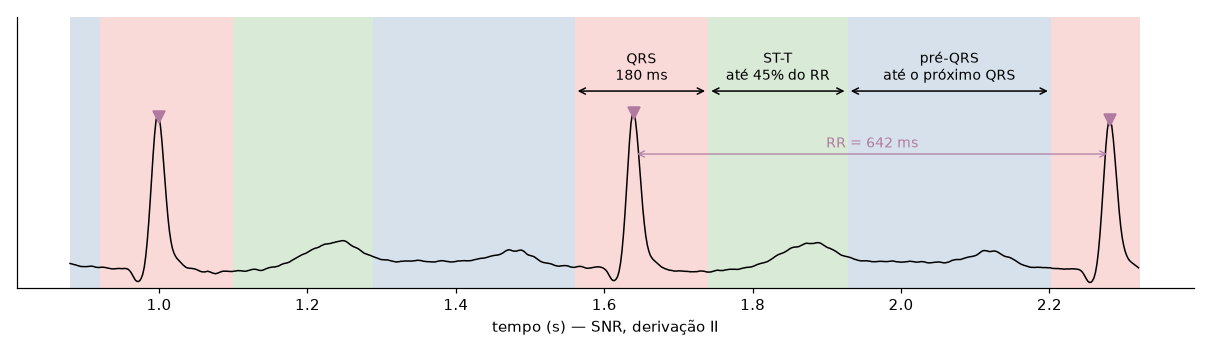
\includegraphics[width=0.85\textwidth]{figs/batimento.png}
\caption{Trecho de cerca de 1,5 s da derivação II de um ECG normal, com três picos R (triângulos) e as regiões de cada batimento: QRS (vermelho), ST-T (verde) e pré-QRS (azul). As mesmas regiões são aplicadas às 12 derivações.}
\label{fig:regioes}
\end{figure}

\subsection{Sufficiency: retirada}
O artigo que a define (Dasgupta et al., 2022) afirma que, para métodos de importância de atributos como o SHAP, não é possível saber quando uma explicação “se aplica” a outro exemplo, e por isso não define a métrica para esses métodos. A versão do Quantus compara mapas por distância, o que na prática é uma segunda Consistency, sem base na definição original.

\subsection{Consistency: reimplementada}
\textbf{O problema.} A discretização padrão do Quantus usa o sinal dos 5 \emph{primeiros} valores do mapa (e não dos 5 mais importantes), depois de aplicar valor absoluto. Nos mapas do projeto, isso deu \textbf{a mesma explicação para todos os ECGs}, e a métrica passava a medir só a homogeneidade das predições.

\textbf{A versão atual.} Segue a definição e o estimador de Dasgupta et al. (2022): a explicação de cada mapa é o par das 2 regiões mais importantes, com o sinal; para cada mapa, calcula-se a fração dos outros mapas com a mesma explicação que explicam a mesma classe. O valor esperado ao acaso é reportado como referência.

\subsection{Faithfulness Correlation: reimplementada}
\textbf{O problema.} O Quantus retira 224 pontos isolados (0,12\% do sinal) e os substitui pelo valor mínimo do próprio ECG. Num diagnóstico com 36 ECGs, essa perturbação mudou bastante a saída do modelo, mas \textbf{sem relação com as atribuições} (correlação média de $-$0,02): a queda refletia os picos artificiais criados pelo valor mínimo, e não a retirada de informação.

\textbf{A versão atual.} Segue o protocolo de Bhatt et al. (2020): para cada ECG, sorteiam-se 50 grupos de regiões; para cada grupo, compara-se a soma das atribuições com a queda do \textit{logit} da classe ao substituir as regiões pela baseline. O valor do ECG é a correlação de Pearson entre essas duas listas. Como no artigo, foram usadas as baselines zero e média do treino (que deram resultados praticamente iguais) e vários tamanhos de grupo (4, 9 e 18 regiões). No mesmo diagnóstico, a correlação média passou de $-$0,02 para 0,57.

As duas implementações foram conferidas em casos sintéticos com resultado conhecido, e cada métrica tem um fichamento do artigo original com a comparação artigo × Quantus × versão atual.

\section{Resultados (modelo B)}

\begin{table}[H]
\centering
\small
\caption{F1, Consistency e Faithfulness Correlation por classe. Entre parênteses, a posição da classe em cada medida (1º = maior valor).}
\label{tab:res}
\begin{tabular}{lr rr rr rr}
\toprule
\textbf{Classe} & \textbf{Mapas} & \multicolumn{2}{c}{\textbf{F1}} & \multicolumn{2}{c}{\textbf{Consistency (acaso)}} & \multicolumn{2}{c}{\textbf{Faithfulness Corr.}} \\
\midrule
BRD  & 172 & 0,927 & (2º) & 0,64 (0,23) & (1º) & 0,74 & (1º) \\
IAVB &  61 & 0,884 & (3º) & 0,45 (0,08) & (3º) & 0,64 & (3º) \\
AF   & 108 & 0,931 & (1º) & 0,42 (0,14) & (4º) & 0,54 & (6º) \\
CVP  &  59 & 0,837 & (5º) & 0,26 (0,08) & (5º) & 0,61 & (4º) \\
BRE  &  20 & 0,870 & (4º) & 0,25 (0,03) & (6º) & 0,65 & (2º) \\
STD  &  65 & 0,778 & (7º) & 0,51 (0,09) & (2º) & 0,52 & (7º) \\
SNR  &  78 & 0,796 & (6º) & 0,21 (0,10) & (7º) & 0,46 & (9º) \\
CAP  &  45 & 0,750 & (8º) & 0,14 (0,06) & (8º) & 0,52 & (8º) \\
STE  &  14 & 0,596 & (9º) & 0,03 (0,02) & (9º) & 0,60 & (5º) \\
\midrule
\textbf{Global} & 622 & \textbf{0,819} & & \textbf{0,42 (0,13)} & & \textbf{0,61} & \\
\bottomrule
\end{tabular}
\end{table}

\begin{figure}[H]
\centering
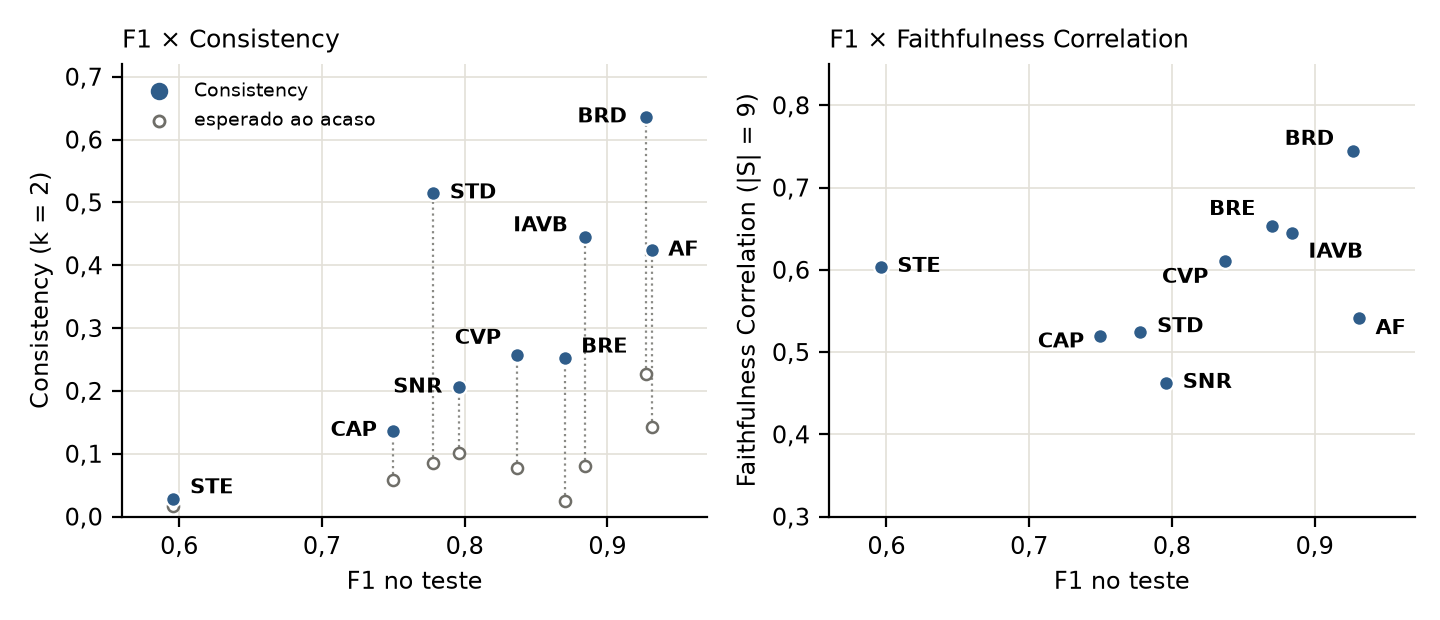
\includegraphics[width=0.95\textwidth]{figs/f1_vs_metricas.png}
\caption{F1 por classe contra a Consistency (esquerda; círculos vazios: valor esperado ao acaso) e contra a Faithfulness Correlation com grupos de 9 regiões (direita).}
\label{fig:disp}
\end{figure}

\section{Conclusões até agora}

As comparações com o F1 são \textbf{descritivas} (ordenação das classes), sem coeficientes de correlação: as nove classes não são observações independentes (registros multirrótulo, mesmo modelo e mesmo conjunto de teste) nem uma amostra de uma população maior de classes.

\begin{enumerate}
    \item \textbf{As explicações SHAP carregam informação real sobre o modelo.} A Consistency global (0,42) é cerca de três vezes o esperado ao acaso (0,13), e a Faithfulness Correlation (0,61) é positiva em todas as classes: quando o SHAP aponta um grupo de regiões como mais importante, retirá-lo derruba mais a saída do modelo. Os valores são moderados, e não perfeitos.
    \item \textbf{BRD tem as explicações de melhor qualidade} nas duas métricas (1º em ambas) e está entre as classes de maior F1. As regiões que o SHAP destaca coincidem com o critério clínico (QRS em V1/V2).
    \item \textbf{CAP fica na base nas três medidas} (8º no F1, na Consistency e na Faithfulness Correlation), e \textbf{IAVB} fica em 3º nas três.
    \item \textbf{Desempenho e qualidade das explicações coincidem nas pontas, mas não de forma estrita.} Há discordâncias: AF tem o melhor F1 e qualidade intermediária; STE tem o pior F1, Consistency quase nula e Faithfulness Correlation intermediária (com só 14 mapas); STD tem explicações muito consistentes, mas fidelidade intermediária.
    \item \textbf{As duas métricas medem propriedades diferentes} e nem sempre concordam entre si (por exemplo, STD e BRE), o que reforça a importância de avaliar a qualidade das explicações por mais de uma dimensão.
    \item \textbf{A configuração padrão do Quantus não pode ser usada sem revisão} no caso do ECG: nas duas métricas revisadas, ela produzia resultados que não refletiam as explicações.
\end{enumerate}

\textbf{Limitações:} um único modelo e uma única divisão dos dados; apenas as predições corretas foram explicadas; classes pequenas (STE, BRE) têm valores menos estáveis; as métricas medem a coerência das explicações com o modelo, e não a sua correção clínica.

\section{Revisão das demais métricas}

As métricas restantes estão sendo revisadas com o mesmo procedimento usado para a Consistency e a Faithfulness Correlation: (1) leitura do artigo original; (2) comparação da implementação e da configuração do Quantus com a definição; (3) se houver dúvida, um diagnóstico com dados; (4) se necessário, reimplementação adaptada ao ECG; (5) fichamento documentando as decisões.

\begin{table}[H]
\centering
\small
\caption{Situação das métricas.}
\begin{tabularx}{\textwidth}{lXl}
\toprule
\textbf{Métrica} & \textbf{Artigo de referência} & \textbf{Situação} \\
\midrule
\multicolumn{3}{l}{\textit{Fidelidade}} \\
Consistency & Dasgupta, Frost e Moshkovitz (2022) & Reimplementada e calculada \\
Faithfulness Correlation & Bhatt, Weller e Moura (2020) & Reimplementada e calculada \\
Sufficiency & Dasgupta, Frost e Moshkovitz (2022) & Retirada \\
Faithfulness Estimate & Alvarez-Melis e Jaakkola (2018) & Próxima a revisar (artigo já baixado) \\
Sensitivity-N & Ancona et al. (2018) & A revisar (artigo já baixado) \\
Selectivity & Montavon, Samek e Müller (2018) & A revisar; estourava a memória (RAM) \\
Infidelity & Yeh et al. (2019) & A revisar; a mais cara de calcular \\
\midrule
\multicolumn{3}{l}{\textit{Robustez}} \\
Local Lipschitz Estimate & Alvarez-Melis e Jaakkola (2018) & A revisar; estourava a memória da GPU \\
Max- e Avg-Sensitivity & Yeh et al. (2019) & A revisar; estouravam a memória da GPU \\
Continuity & Montavon, Samek e Müller (2018) & A revisar; estourava a memória da GPU \\
RIS e ROS & Agarwal et al. (2022) & A revisar; estouravam a memória da GPU \\
\bottomrule
\end{tabularx}
\end{table}

\section{Próximos passos}
\begin{itemize}
    \item Revisar a Faithfulness Estimate e a Sensitivity-N, cujos artigos já foram baixados, seguidas das demais métricas de fidelidade.
    \item Revisar as métricas de robustez, resolvendo também os problemas de memória da GPU.
    \item Calcular cada métrica revisada sobre o modelo B, reaproveitando o modelo e os mapas já gerados, e acrescentá-la à comparação descritiva com o F1.
\end{itemize}

\end{document}
